%!TEX root = ../thesis.tex
%*******************************************************************************
%*********************************** First Chapter *****************************
%*******************************************************************************

\chapter{Analysing the problem}  %Title of the First Chapter

\ifpdf
    \graphicspath{{Chapter1/Figs/Raster/}{Chapter1/Figs/PDF/}{Chapter1/Figs/}}
\else
    \graphicspath{{Chapter1/Figs/Vector/}{Chapter1/Figs/}}
\fi


%********************************** %First Section  **************************************

\section{Defining the problem itself} %Section - 1.1 

Warehouses often employ several workers for menial labour jobs such as the retrieval of thousands of items over the space of an average day. This business model is impractical due to the costs of hiring warehouse workers and managers for such simple tasks as noting stock levels and collecting items. My project aims to optimise warehouse operations through a \textbf{hypothetical} robot - the StockBot. It will retrieve multiple stock items at a time, finding the shortest path required to collect all items and reach its destination. The program will utilise a path-finding algorithm to trace the most optimal path to pick up items and drop off at a fixed location, while cross-referencing a database to ensure items are in stock. I envision this to be applied in a warehouse or alternative bulk storage facility, such as that of an e-commerce business. My solution reduces business costs and improves efficiency, removing a large portion of human operations and replacing them with autonomous workers.

\begin{figure}[h!] 
\centering    
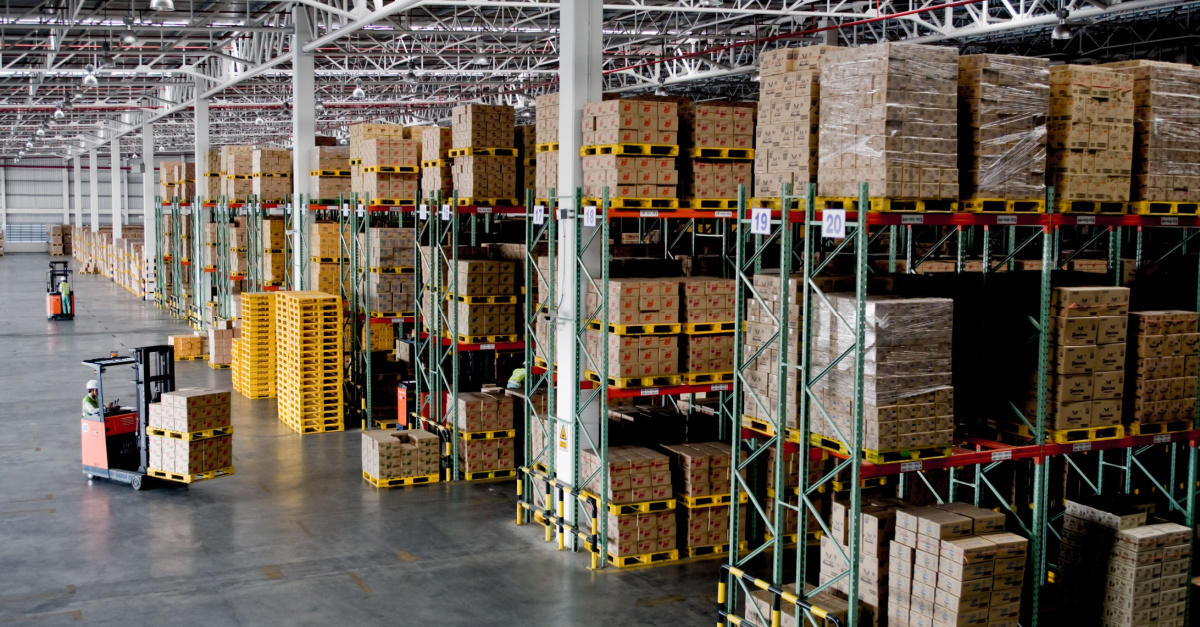
\includegraphics[width=0.8\textwidth]{Images/warehouse.jpg}
\caption{- A sample warehouse environment. \cite{warehouse}}
\end{figure}

\newpage

%********************************** %Second Section  *************************************
\section{Current systems model} %Section - 1.2

The current process model for a warehouse worker typically involves receiving orders, compiling product lists, collecting items from designated locations, and placing them in shipping areas.\newline \textbf{}\newline While this manual process is feasible for smaller operations, it becomes increasingly inefficient and error-prone as the scale of the warehouse expands. Human workers are susceptible to errors, such as picking incorrect items or placing them in the wrong locations. Manual processes can also be time-consuming, especially for large orders or complex warehouses. Additionally, repetitive tasks like collecting and placing products can lead to fatigue and reduced productivity. These factors contribute to higher operational costs and potential delays in order fulfilment. \newline \textbf{}\newline The limitations of human workers can be addressed through automation; robots can perform these tasks with greater accuracy and efficiency, reducing the risk of errors and improving overall productivity. Unlike humans, robots can operate continuously without breaks or rest, enabling 24/7 operations. \newline \textbf{}\newline While the initial investment in robotic technology may be higher, the long-term cost savings from reduced labour and improved efficiency can make it a worthwhile investment. Furthermore, robots can enhance workplace safety by handling hazardous materials or performing tasks in dangerous environments. This reduces the risk of injuries to human workers and improves overall safety standards within the warehouse.
\begin{figure}[h]
    \centering
    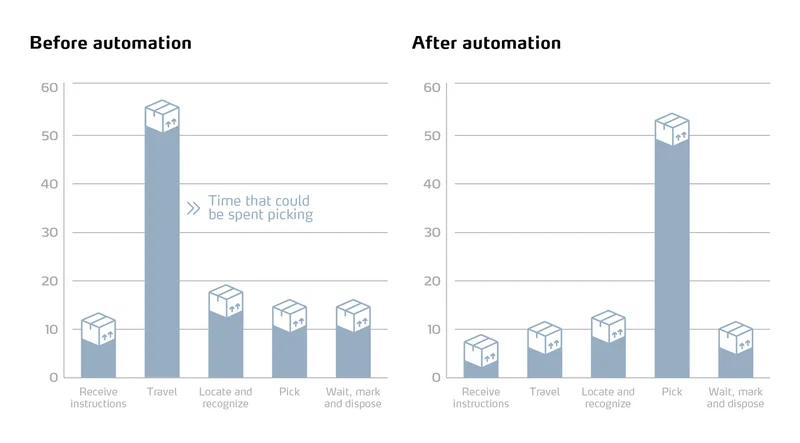
\includegraphics[width=0.8\linewidth]{automation+.png}
    \caption{ - Automation benefits \cite{warehouseauto}}
\end{figure}


\newpage

As you can see in Figure 1.3, the current model of a warehouse worker seems less complex than a computational approach, however the focus is not on the size or number of elements, but rather the time taken to complete each task. While a computational approach may have more tasks, it can complete them in a much shorter time, leading to better efficiency.

\begin{figure}[h] 
\centering    
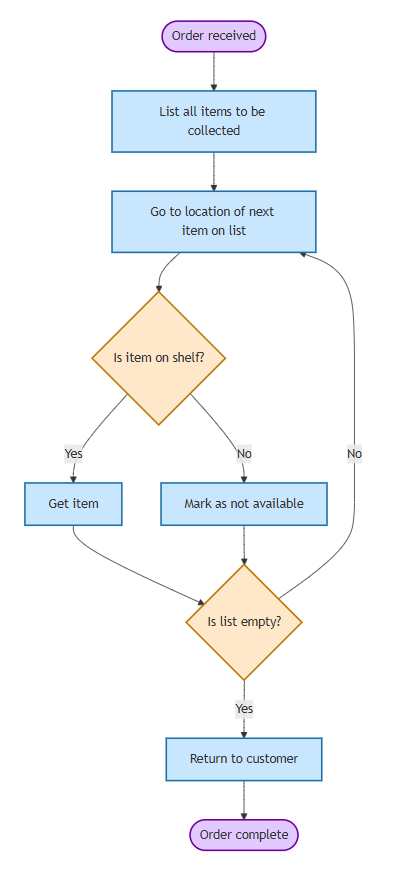
\includegraphics[width=0.5\textwidth]{CurrentSysModel.png}
\caption{- The current process of a warehouse worker}
\label{The current process of a warehouse worker}
\end{figure}

\newpage

\section{Computational methods}

This problem is well suited for a computer as there is a valid and usable solution using computational methods. StockBot can perform operations much more efficiently than a human, as these are menial tasks requiring minimal thinking power but rather a continual set of instructions to perform certain tasks \textbf{and those tasks only}, a framework which computers excel at. Below I have listed justifications of a computational approach to this problem.

\subsection{Thinking Abstractly}
Since this is not an industrial project, I will need to decide what aspects of the solution I can remove to make my program more appropriate, keeping only the features that are necessary. Initially, these are the abstractions I proposed, which I will consider with my stakeholders:

\begin{itemize}
    \item Restrict warehouses to 2 dimensions: 3D warehouses will be difficult to represent or visualise, and adds unnecessary complexity as items are often grouped vertically, meaning from a 2D perspective they are all located at that position, regardless of height.

    \item Grid layout only: most warehouses are grids for optimal storage capacity. I felt that the extremely small minority without such a layout would not benefit from the solution, hence a focus on rectangular formats only.

    \item Simple visualisations: Too complex GUIs can lead to unnecessary complexity and cognitive overload, therefore I will be focussing on creating an interface with only the functions I implement (while still maintaining usability), with little else in terms of design.
\end{itemize}

\subsection{Thinking Ahead}

I plan to use Python to develop my solution, due to its versatility and easy-to-understand syntax as a high-level language. When developing my program, I aim to follow an object-oriented approach, as it allows for simplified debugging, excellent organisation and reducing duplicate code snippets (the method can just be called again.) See below for a table of technologies I aim to use.


\begin{table}[h]
\centering
\begin{tabular}{|p{3cm}|p{5cm}|p{6cm}|}
\hline
\textbf{Tech} & \textbf{Summary} & \textbf{Justification} \\
\hline
Python & High-level programming language & Versatile, easy-to-understand language \\
\hline
Object-Oriented Programming & Programming paradigm focusing on objects & Simplifies debugging, enables code reuse and improves organisation \\
\hline
SQLite & Lightweight SQL database & Integrates well with Python, easy storage solution \\
\hline
Tkinter & Python GUI library & Creates a user-friendly, easy to understand interface for my program\\
\hline
\end{tabular}
\end{table}

\subsection{Thinking Procedurally}

I plan to break my solution down into 3 main components for the final solution - this is most likely how my file structure will be split:
\begin{itemize}
    \item Shortest Path Algorithm - this is the central part of the program, the back-end which makes the program useful.
    \item User interaction - this will be all sub-components relating to how the user interacts with the program, from the GUI to help menus and so on.
    \item Database operations - this will be for managing the warehouse in which the program is operating in.
\end{itemize}

\subsection{Thinking Logically}

This focuses on the more logical aspect of my program, i.e. ensuring not only my approach is logical but also features of my program are understandable and each feature has unique characteristics: this prevents duplication and unnecessary code being written.

\subsection{Thinking Concurrently}
This will be useful for determining what operations or sub-programs should be running at any given time, and how I can optimise my program for faster usage times.



\section{Stakeholders in a solution} 

\subsection{Stakeholder definition}

My end user for such a product could hypothetically be any business, small or large, that uses warehouses or other organised storage systems. For example, an e-commerce business could benefit from a robotic worker to efficiently pack multiple orders.
\textbf{\newline}
\newline
In my case, my father will be the primary stakeholder - he works for Currys, where I have seen first-hand the day-to-day warehouse operations as well as possible improvements that could be made to the current model. My secondary stakeholders are 2 teachers, Mr Ryan Slater and Mr Alex Johnson, both of whom have taken a vested interest in this project.
\newline
To evaluate which features they would require, I will conduct some interviews and questionnaires to build the best possible product and implement the most relevant features.


\subsection{Stakeholder use of solution}

My father will be able to use the stock robot to:

\begin{itemize}
    \item \textbf{Automate repetitive tasks:} The robot will take over tasks like retrieving stock and keeping track of inventory, freeing up employees to focus on more complex tasks.
    \item \textbf{Improve efficiency:} The robot will be able to work faster and more accurately than humans, leading to increased productivity and faster management, meaning that new stock can be ordered much more quickly.
    \item \textbf{Reduce errors:} The robot will be able to scan stock codes and verify items, reducing the risk of retrieving the incorrect item.
    \item \textbf{Improve safety:} The robot will be able to navigate the warehouse in a safer manner compared to a human, and could eliminate the risk of injury from items falling from shelves.
\end{itemize}


\newpage

\section{Investigation}

\subsection{Primary Stakeholder Data}

As a worker of Currys, my father is often required to retrieve many items over the course of his work-day, and he often takes up to 20 mins to find an item. To address this problem, I intend to collect information through my father over the course of a work week to address the most critical issues he faces, and consult my secondary stakeholders for confirmation and extra ideas.

\subsubsection{Data collection}

From my father, I will be collecting the time taken to process a customer's request for an item. I will take 5 samples out of his day across 5 days, totalling 25 interactions. I feel this is an appropriate sample to judge current operations in his workplace. \newline

\textbf{Categories:}

\begin{enumerate}
    \item Warehouse: Time taken to reach the warehouse from a random point in the store. While my project may not have a significant impact on this time as it will be operating elsewhere, I felt it necessary to gain a full picture from start to end.

    \item Locate: Time taken to locate the item that the customer is requesting. This is what StockBot will have a significant impact on in terms of optimising business operations and efficiency.

    \item Return: Time taken to return the item requested to the customer. StockBot should have medium impact on this, as workers can simply wait by the doors of the warehouse rather than having to walk in and out.
\end{enumerate}

\subsubsection{Gathered data}

\begin{table}[htbp]
\centering
\small
\begin{tabular}{|c|c|c|c|c|c|}
\hline
\textbf{Day} & \textbf{\#} & \textbf{Warehouse} & \textbf{Locate} & \textbf{Return} & \textbf{Total} \\
\hline
\multirow{5}{*}{Mon} & 1 & 2:14 & 7:36 & 2:05 & 11:55 \\
& 2 & 3:25 & 5:42 & 2:38 & 11:45 \\
& 3 & 2:52 & 10:15 & 2:33 & 15:40 \\
& 4 & 3:12 & 7:18 & 1:47 & 12:17 \\
& 5 & 2:38 & 8:12 & 2:25 & 13:15 \\
\hline
\multirow{5}{*}{Tue} & 1 & 4:03 & 6:22 & 3:10 & 13:35 \\
& 2 & 2:45 & 5:38 & 2:12 & 10:35 \\
& 3 & 3:18 & 9:45 & 3:07 & 16:10 \\
& 4 & 2:59 & 6:53 & 2:43 & 12:35 \\
& 5 & 3:42 & 7:15 & 2:21 & 13:18 \\
\hline
\multirow{5}{*}{Wed} & 1 & 3:27 & 5:13 & 3:05 & 11:45 \\
& 2 & 2:49 & 11:33 & 2:38 & 17:00 \\
& 3 & 3:05 & 8:07 & 1:55 & 13:07 \\
& 4 & 3:37 & 6:48 & 2:15 & 12:40 \\
& 5 & 2:42 & 7:19 & 2:32 & 12:33 \\
\hline
\multirow{5}{*}{Thu} & 1 & 3:52 & 6:45 & 2:57 & 13:34 \\
& 2 & 2:38 & 9:12 & 1:58 & 13:48 \\
& 3 & 3:23 & 7:47 & 2:33 & 13:43 \\
& 4 & 4:05 & 8:23 & 3:12 & 15:40 \\
& 5 & 2:51 & 5:19 & 2:07 & 10:17 \\
\hline
\multirow{5}{*}{Fri} & 1 & 3:32 & 7:55 & 2:22 & 13:49 \\
& 2 & 3:48 & 6:38 & 2:41 & 13:07 \\
& 3 & 2:57 & 5:28 & 2:13 & 10:38 \\
& 4 & 3:15 & 8:45 & 2:52 & 14:52 \\
& 5 & 3:08 & 7:12 & 2:37 & 12:57 \\
\hline
\multicolumn{2}{|c|}{\textbf{Average}} & \textbf{3:11} & \textbf{7:31} & \textbf{2:31} & \textbf{13:13} \\
\hline
\end{tabular}

\medskip
\end{table}

\section*{Questionnaire: Primary Stakeholder}

\subsection*{Purpose}
This questionnaire is designed to gather detailed insights from my father. The goal is to understand the challenges he faces in his daily tasks and how the proposed solution can address these issues effectively.

\subsection*{Section 1: Current Challenges}

\begin{enumerate}
    \item \textbf{How much time do you typically spend searching for an item in the warehouse?}
    \begin{itemize}
        \item Less than 5 minutes
        \item \textbf{\underline{5–10 minutes}}
        \item 10–20 minutes
        \item More than 20 minutes
    \end{itemize}

    \item \textbf{What are the most common difficulties you face when searching for items manually?} (Select all that apply)
    \begin{itemize}
        \item \textbf{\underline{Items are misplaced or not where they should be}}
        \item Difficulty navigating the warehouse layout
        \item Lack of real-time stock information
        \item \textbf{\underline{Fatigue from walking long distances}}
        \item Other (please specify): \underline{\textbf{Large warehouse means long search times}}
    \end{itemize}

    \item \textbf{How often do you encounter situations where an item is out of stock or unavailable?}
    \begin{itemize}
        \item \textbf{\underline{Rarely}}
        \item Occasionally
        \item Frequently
    \end{itemize}

    \item \textbf{How do you currently track or verify stock levels before retrieving an item?}
    \begin{itemize}
        \item Manual counting
        \item Checking a paper-based inventory list
        \item \textbf{\underline{Using a digital system (if applicable, please describe): }}\underline{\textbf{Proprietary software}}
        \item No formal process
    \end{itemize}

    \item \textbf{Is the tracking method outlined above accurate?}
    \begin{itemize}
        \item Rarely
        \item Occasionally
        \item \textbf{\underline{Most of the time}}
        \item All of the time
    \end{itemize}

    \item \textbf{On average, how many items do you retrieve in a single trip to the warehouse?}
    \begin{itemize}
        \item \textbf{\underline{1–5 items}}
        \item 6–10 items
        \item More than 10 items
    \end{itemize}
    
    \newpage

    \item \textbf{Have you explored the possibility of an automated workforce in the warehouse?}
    \begin{itemize}
        \item \textbf{\underline{Yes}}
        \item No
        \item Unsure
    \end{itemize}

    \item \textbf{If yes, why was it not implemented?}
    \begin{itemize}
        \item \textbf{\underline{Cost}}
        \item \textbf{\underline{Lack of justifiable benefits}}
        \item Poor usability
        \item Bad user experience
        \item Prefer not to disclose
    \end{itemize}

    \item \textbf{What is a necessity to even consider this solution?}
    \begin{itemize}
        \item \textbf{\underline{Faster collections}}
        \item Good usability
        \item Scalability
    \end{itemize}
\end{enumerate}

\subsection*{Section 2: Potential Improvements}

\begin{enumerate}
    \item \textbf{If a system could automatically check stock availability before you search for an item, how useful would you find this feature?}
    \begin{itemize}
        \item \textbf{\underline{Very useful}}
        \item Somewhat useful
        \item Not useful
    \end{itemize}

    \item \textbf{Would obstacle avoidance have a large impact on your warehouse?}
    \begin{itemize}
        \item Yes, significantly
        \item \textbf{\underline{Yes, but only slightly}}
        \item No, it wouldn’t make a difference
    \end{itemize}

    \item \textbf{How important is it for the system to provide real-time updates on your progress (e.g., which items have been collected, remaining items)?}
    \begin{itemize}
        \item Very important
        \item \textbf{\underline{Moderately important}}
        \item Not important
    \end{itemize}

    \item \textbf{How important is it for the system to provide real-time updates on progress (e.g., which items have been collected, remaining items)?}
    \begin{itemize}
        \item Very important
        \item \textbf{\underline{Moderately important}}
        \item Not important
    \end{itemize}

\end{enumerate}

\subsection*{Section 3: Usability}

\begin{enumerate}
    \item \textbf{How comfortable are you using digital tools (e.g., apps, software) for work-related tasks?}
    \begin{itemize}
        \item \textbf{\underline{Very comfortable}}
        \item Somewhat comfortable
        \item Not comfortable
    \end{itemize}

    \item \textbf{How important is it for the system to have a simple and intuitive interface?}
    \begin{itemize}
        \item \textbf{\underline{Very important}}
        \item Moderately important
        \item Not important
    \end{itemize}

    \item \textbf{How frequently would you use such a system if it were available?}
    \begin{itemize}
        \item \textbf{\underline{Every day}}
        \item A few times a week
        \item Rarely
    \end{itemize}
    
\end{enumerate}


\subsection*{Other comments:}

It simply should speed up our processing times. Customers often complain that they aren't receiving their items quick enough, and in some cases decide to leave and go elsewhere. Your software should aim to speed up our process so we can retain and serve more customers.\newline

Usability is key: we don't want to waste time training new employees how to use the software. Because we don't have strict requirements for qualifications, we get a range of people with varying capabilities, and we don't want to spend time explaining intricacies, bugs and common issues: we need something that just works and is self-explanatory.\newline

I think the primary feature should be the path-finding algorithm. It's what will have the most impact on us, since our main problem is timing. Obstacle placement would also be useful as we often do have obstacles like piled-up crates. Anything else is secondary to everything else mentioned - main features should be quick pathfinding, obstacle placement, easy-to-use interface and some sort of feedback.
\vspace{2cm}
\newline
\textbf{\underline{Minash Khambhaita}} \newline
Employee @ Currys PLC

\newpage
\subsection{Secondary Stakeholder Questionnaire \& Responses}

\subsection*{Purpose}
This questionnaire is designed to gather feedback from my secondary stakeholders (teachers) on the features and usability of the proposed solution. The goal is to ensure the project aligns with client expectations as well as offer excellent usability. As such, this questionnaire focuses more on usability features as well as assessing whether possible features presented to them would be of use and as such incorporated into the solution.

\subsection*{Section 1: General Feedback}

\begin{enumerate}
    \item \textbf{Based on the project outline, which feature do you think is most critical for the success of the system?}
    \begin{itemize}
        \item Stock checker (verifies stock availability before retrieval)
        \item \textbf{\underline{Shortest path algorithm (calculates the fastest route to collect items)}}
        \item Direct feedback (provides real-time updates on progress)
        \item Graphical User Interface (GUI) for ease of use
    \end{itemize}

    \item \textbf{How important is it for the system to integrate with a database for managing stock levels?}
    \begin{itemize}
        \item Very important
        \item \textbf{\underline{Moderately important}}
        \item Not important
    \end{itemize}

    \item \textbf{Which aspect of the system do you think would benefit the client the most?}
    \begin{itemize}
        \item \textbf{\underline{Algorithm efficiency (e.g., finding the shortest path)}}
        \item Database management (e.g., updating stock levels)
        \item User interface design (e.g., ease of use, visual clarity)
        \item Error handling (e.g., dealing with invalid inputs or out-of-stock items)
    \end{itemize}

    
\end{enumerate}


\subsection*{Section 2: Feature Prioritisation}

\begin{enumerate}
    \item \textbf{How useful would it be for the system to allow users to input multiple waypoints (locations of items) at once?}
    \begin{itemize}
        \item \textbf{\underline{Very useful}}
        \item Somewhat useful
        \item Not useful
    \end{itemize}

    \item \textbf{Would you prioritise a system that focuses on simplicity or one that includes advanced features (e.g., handling weighted paths, dynamic obstacles)?}
    \begin{itemize}
        \item \textbf{\underline{Simplicity}}
        \item Advanced features
    \end{itemize}

    \item \textbf{How important is it for the system to provide visual feedback (e.g., a grid showing the warehouse layout and path)?}
    \begin{itemize}
        \item \textbf{\underline{Very important}}
        \item Moderately important
        \item Not important
    \end{itemize}

    \item \textbf{Should the system include a help section or tooltips to guide users through its features?}
    \begin{itemize}
        \item Yes, very important
        \item \textbf{\underline{Yes, but only moderately important}}
        \item No, not necessary
    \end{itemize}
\end{enumerate}

\subsection*{Section 3: Usability and Design}

\begin{enumerate}
    \item \textbf{How important is it for the system to follow established usability guidelines (e.g., visibility of system status, error prevention)?}
    \begin{itemize}
        \item \textbf{\underline{Very important}}
        \item Moderately important
        \item Not important
    \end{itemize}

    \item \textbf{How important is it for the system to be scalable (i.e., adaptable to larger warehouses or more complex operations)?}
    \begin{itemize}
        \item Very important
        \item \textbf{\underline{Moderately important}}
        \item Not important
    \end{itemize}
\end{enumerate}

\subsection*{Other comments:}

We agree that the shortest path algorithm is critical to the solution, without it the program is useless. It should aim to be efficient enough to be a good replacement for current operations. Integration with a database could be good, but it is not as essential. If it can be done, then excellent. Same with scalability, it is excellent to have but your program should aim to be usable first-and-foremost. Also, you might want to look at a way that people can input their own data quickly, as I guess manually filling out inventory levels is quite time-consuming
\vspace{0.7cm}
\newline

\textbf{\underline{Mr Ryan Slater \& Mr Alex Johnson}} \newline


\newpage

\subsection{Conclusion}

Based on the feedback received, I will focus on simplicity rather than overly complex features, ensuring that StockBot provides greater value through faster collection times rather than more features which are already available and not unique. The time measurements I collected provide a clear baseline against which I can measure StockBot's performance. My goal is to substantially reduce the average time of 7:31 minutes to locate and retrieve an item, which will directly address my primary stakeholder's concern of losing customers due to timing.

\subsubsection{Primary Features}

\begin{enumerate}
    \item \textbf{Advanced Pathfinding Algorithm}\\
    My research shows that implementing an efficient pathfinding algorithm must be my highest priority. Both my father (primary stakeholder) and my teachers (secondary stakeholders) emphasised this as the most critical component. The time data collected over 5 days confirms this need, with locating items consistently taking the longest time across all 25 recorded interactions.
    
    I will implement a pathfinding algorithm that can:
    \begin{itemize}
        \item Calculate the optimal route between multiple item locations
        \item Generate the shortest possible path to minimise collection time
        \item Operate efficiently within the warehouse's layout constraints
    \end{itemize}
    
    \item \textbf{Intuitive Graphical User Interface}\\
    The primary stakeholder emphasised that ``usability is key'' and that the system must be ``self-explanatory'' for employees with varying technical abilities. The interface will include:
    \begin{itemize}
        \item Visual representation of the warehouse layout
        \item Simple controls for entering item locations
        \item Colour-coding for each item
    \end{itemize}
    
    \item \textbf{Multi-Item Collection Capability}\\
    The data reveals that employees typically retrieve 1-5 items per warehouse trip. Enabling StockBot to handle multiple items in a single operation will significantly reduce the overall time spent. This feature was rated as ``very useful'' by the secondary stakeholders and will address my father's concern about collection times.
\end{enumerate}

\subsubsection{Secondary Features}

\begin{enumerate}
    \item \textbf{Database Integration}\\
    While my father indicated that the current proprietary stock system is accurate ``most of the time,'' integrating StockBot with a database will enhance its functionality. Benefits:
    \begin{itemize}
        \item Store item locations for quick retrieval
        \item Maintain a record of stock levels for verification
        \item Support future expansions of the system's capabilities
    \end{itemize}
    
    \item \textbf{Progress Tracking}\\
    Real-time updates on collection progress were rated as ``moderately important'' by my father. Implementing this feature will provide valuable feedback during the collection process and help address his concern that ``customers often complain that they aren't receiving their items quick enough.''
    
    \item \textbf{Minimal Help System}\\
    A simple help system was rated as ``moderately important'' by the secondary stakeholders. This aligns with my father's requirement for a system that ``just works.'' I will include detailed help tooltips within the interface, as well as a brief guide to ensure new users can quickly understand the system without extensive training.
\end{enumerate}

\subsubsection{Desirable/Optional Features}

\begin{enumerate}
	\item \textbf{JSON Import/Export}\\
	My secondary stakeholders mentioned that some sort of way to input data other than the interface/manually could be good: hence I settled on a JSON import and export feature, where data is saved to a file and can be inputted/outputted easily.
	
	\item \textbf{Output as image}\\
	My father mentioned that usability is essential: I think it would be useful if the path could be printed as an image so that it can also be manually followed and provides an easy reference.
	
	\item \textbf{Path animation}\\
	As usability is key for this software, a path animation could be a method of easily following the path as it is constructed, and is an abstraction of an actual robot moving in the warehouse.
	
\end{enumerate}


Based on the research into both current implementations and shortest path algorithms I will conduct, I will make an informed decision about what I believe are the best features and algorithm(s) to incorporate into the final solution from this larger list. Not all of these features listed above will be included, as I plan to refine this into a fixed set of features that would benefit the client the most.